% Copyright (C) 2012 by Werner Moshammer
% This file may be distributed and/or modified under the LaTeX Project Public License

%\documentclass[11pt]{article}
\documentclass[a4paper]{ltxdoc}

\usepackage{tikz}
\usetikzlibrary{arrows,automata}

\usepackage{hyperref}
\hypersetup
{
    pdfauthor={Di Werner Moshammer},
    pdfsubject={The ocg-p package},
    pdftitle={The ocg-p package},
    pdfkeywords={LaTeX,OCG, Layers}
}


\usepackage{fancyvrb}
%\usepackage{ocg-p}
\usepackage{framed}

\usepackage{datatool} 
\usepackage{booktabs}




\usepackage{listings}
%\usepackage{xcolor}

\lstset{
  language=[LaTeX]TeX,
  basicstyle=\footnotesize\ttfamily,
  upquote=true,
  frame=single,
  keywordstyle=\color{blue}\bfseries,
  emphstyle=\color{blue}\bfseries,
  backgroundcolor=\color{black!05},
  fontadjust=true,
  flexiblecolumns=true,
  breaklines=true, 
  emph={ocg}
}

\newcommand{\TikZ}{Ti\emph{k}Z}

\newcommand*{\pkg}[1]{\textsf{#1}}
\newcommand*{\mail}[1]{\href{mailto:#1}{\texttt{#1}}}

\ifpdf
\pdfinfo{
/Author (DI Werner Moshammer)
/Title (The ocg-p package)
}
\fi

\title{The \pkg{ocg-p} package\thanks{This manual correspondends to \pkg{ocg-p} v0.4, dated 2013/01/10}}
\author{DI Werner Moshammer\thanks{Contact me when you find mistakes in the manual: \mail{sendmail.werner@gmail.com}}}
\date{2013/01/10}

\begin{document}

\maketitle

\tableofcontents



\begin{abstract}
The \pkg{ocg-p} package provides the environment that allows to insert OCG (Optional Content Group) into PDF documents without JavaScript. These OCGs can be simply described as layers from the user's point of view. 

The \pkg{ocg-p} package is intended as a full replacement for the file |ocg.sty| which is part of the \pkg{asymptote} package. While |ocg.sty| is limited to be used with |pdfLaTeX|, the \pkg{ocg-p} package can also be used with |XeLaTeX|. Additionally nested OCGs (layers inside of another layer) are handled as such.

\end{abstract}
\newpage

\section{Introduction}
The \pkg{ocg-p} package provides the environment that allows to insert OCG (Optional Content Group) into PDF documents without JavaScript. These OCGs can be simply described as layers from the user's point of view.

OCGs are part of the PDF specification since version 1.5 and are described in the \href{http://wwwimages.adobe.com/www.adobe.com/content/dam/Adobe/en/devnet/pdf/pdfs/pdf_reference_archives/PDFReference15_v5.pdf}{PDF Reference} as:

\begin{quote}
Optional content (PDF 1.5) refers to sections of content in a PDF document that
can be selectively viewed or hidden by document authors or consumers. This capability
is useful in items such as CAD drawings, layered artwork, maps, and
multi-language documents.
\end{quote} 

OCGs are not part of the ISO standard 19005 |PDF/A-1|, but part of the newer |PDF/A-2| standard.

The \pkg{ocg-p} package is intended as a full replacement for the file |ocg.sty| which is part of the \pkg{asymptote} package. While |ocg.sty| is limited to be used with |pdfLaTeX|, the \pkg{ocg-p} package can also be used with |XeLaTeX|. Additionally nested OCGs (layers inside of another layer) are handled as such.

\section{Usage}
Here is a quick summary of the usage of \pkg{ocg-p}. The package consists of one main environment to create layers and a few commands for buttons to change the visibility of the layers in some way.
Based on the ocg main environment there is an additionally environment available to create tables, which can be sorted by clicking on the headers.

\subsection{Download}
This package is available on CTAN\footnote{The Comprehensive \TeX{} Archive Network \url{http://www.ctan.org/}}:
\begin{description}
\item[\href{ftp://ftp.ctan.org/tex-archive/macros/latex/contrib/ocg-p/ocg-p.sty}{\texttt{CTAN: macros/latex/contrib/ocg-p/ocg-p.sty}}] The source file.
\item[\href{ftp://ftp.ctan.org/tex-archive/macros/latex/contrib/ocg-p/ocg-p.pdf}{\texttt{CTAN: macros/latex/contrib/ocg-p/ocg-p.pdf}}] Documentation.
\end{description}

\subsection{Package}
Just load the package placing
\begin{quote}
   |\usepackage{ocg-p}|
 \end{quote}
in the preamble of your \LaTeX{}  source file. %There are no options available at the moment.
There is only one option available for the package, which can be used to offer an additional environment to create tables which can be sorted by clicking on the headers. In this case load the package with the following line:
\begin{quote}
   |\usepackage[ocgtabular]{ocg-p}|
 \end{quote}

Important: If packages are used, which use the original \pkg{ocg} package then \pkg{ocg-p} should be loaded after these packages. The |ocg| environment from the \pkg{ocg} package is replaced in this case.

The \pkg{ocg} package is using the auxiliary file, so it is maybe necessary to compile your document 2 - 3 times until all layers are shown properly.

%\subsection{Commands and Environments}
\subsection{The ocg environment}
%At the moment the \pkg{ocg-p} package has only one usable environment. 
This is the main environment of the  \pkg{ocg-p} package.
To create a OCG layer you have to use the |ocg| environment with three required arguments. Because it is intended as a replacement for the file |ocg.sty| this command can be used in the same way as it is used in |ocg.sty|.
\begin{verbatim}
\begin{ocg}{layer name}{layer id}{initial visibility}
content ...
\end{ocg}
 \end{verbatim}
The arguments are:
 \begin{itemize} 
 \item \textit{layer name}:
This name is shown in in the layer toolbar of the (PDF) viewer, where the visiblity of the layers can be changed.
 \item \textit{layer id}:
A unique id which is internally used by the OCG environment to reference the layer. Only letters and numbers are allowed
 \item \textit{initial visibility}:
Sets the initial visibility when the document is opend. Only 0 and 1 are allowed (0 for invisible, 1 for visible)
 \item \textit{content}:
The content of the layer itself.
 \end{itemize}

Beginning with \pkg{ocg-p} version 0.4 there are some optional options available to control the behaviour of the specified  layer. Using this options the |ocg| environment is used the following way:
\begin{verbatim}
\begin{ocg}[opt1=val1, opt2=val2, ...]{layer name}{layer id}{initial visibility}
content ...
\end{ocg}
 \end{verbatim}
The options are given in a comma separated list of optionname value pairs.
The usable options are:

\begin{center}\begin{tabular}{lp{9cm}}\hline
|printocg| & This option can be set to the values |always|, |never| and |ifvisible|. The default value is |ifvisible|. It specifies the visibility state of the content in this layer when the document is printed. |ifvisible| means that the layer is printed only if it is visible in the document. |always| means that it is printed always, independent from the current visiblity state in the document, and |never| means that is never printed.\\
|exportocg| & This option can be set to the values |always|, |never| and |ifvisible|. The default value is |ifvisible|. It specifies the state for the content in this layer when the document is exported or saved to a format that does not support layers. |ifvisible| means that the layer is exported only if it is visible in the document.  |always| means that it is exported always independent from the current visiblity state in the document, and |never| means that is never exported.\\
|listintoolbar| & This option can be set to the values |always|, |never| and |iffirstuse|. The default value is |iffirstuse|. |iffirstuse| means that the layer is only displayed in the toolbar when it is first inserted. |always| means that it is displayed every time this layer is inserted again, and |never| means that the layer is never displayed in the toolbar.  \\ 
\hline
\end{tabular}\end{center}

These options can be combined. So if you want for example that a layer can never be displayed in the document but is visible on a printing then you choose |listintoolbar=never|, |printocg=always| and a initial visible of |0| (invisible).

Important: Nested layers do not work with layers which are not visible in the layer toolbar of the browser.

\subsection{The commands of the package}
Beginning with  \pkg{ocg-p} version 0.4 there are a few additional commands available. These commands can be used to add link actions (buttons) to the document, so that the visibility of some layers can be changed in some way. 
In all commands the |ocg|/|layer ids| should be given in a space separated list, and the last argument is for the link object itself.
By default the link object is used by clicking with the mouse on it (mouseup event). But this behaviour can be changed by the optional options. 

The command |toggleocg| can be used to toggle the visible of the given layers i the document.
\begin{verbatim}
\toggleocgs[optional options]{tlayerid1 tlayerid2 ...}{display}
 \end{verbatim}

The command |showocgs| can be used to make the given layers visible in the document.
\begin{verbatim}
\showocgs[optional options]{slayerid1 slayerid2 ...}{display}
 \end{verbatim}

The command |hideocgs| can be used to make the given layers invisible in the document.
\begin{verbatim}
\hideocgs[optional options]{hlayerid1 hlayerid2 ...}{display}
 \end{verbatim}

The command |setocgs| is a combination of the former commands. With |setocgs| it is possible to toggle some layers given as first argument list, to make some layers visible which are given in the second argument list and to make some layers invisible given in the third argument list.

\begin{verbatim}
\setocgs[optional options]{tlayerid1 tlayerid2 ...}
  {slayerid1 slayerid2 ...}{hlayerid1 hlayerid2 ...}{display}
 \end{verbatim}

There is one optional option availabe for all these commands, called |triggerocg|. These option can be set to the following values:
\begin{center}\begin{tabular}{lp{9cm}}\hline
|onareaenter| & Using this value the action is performed by entering the link area with the cursor (a mousover effect).\\
|onareaexit| & Using this value the action is performed when the cursor exits the link area (a mouseout effect).\\
|onmousedown| & Using this value the action is performed when the mouse button is pressed inside the link area (a mousedown effect).\\
|onmouseup| & Using this value the action is performed when the mouse button isreleased inside the link area (a mouseup effect). |onmouseup| is the default value.\\
|allactions| & When this option is used all four trigger events can be used with different ocgs at the same time. To do this four lists of layer ids have to be given in the arguments of the commands. While one ocg layer id list is given as a space separated list, these lists should be comma separated.\\
& For example:\\
& \verb+\toggleocgs[triggerocg=allactions]+\\ & \verb+     {aenid1 aenid2,aexid1,mdid1,muid1}[display}+ \\
& The first list is for mouseover, the second for mouseout the third for mousedown and the last list for mouseup actions.\\
& Another example where only mouseenter and mousedown actions are used:\\
& \verb+\toggleocgs[triggerocg=allactions]+\\ & \verb+    {aenid1 aenid2,,mdid1 mdid2}+\\
\hline
\end{tabular}\end{center}

Important: It is not possible to make an action area inside of another action layer.

%The |ocg|/|layer ids| in all commands should be given in a space separated list. With |setocgs| it is possible to toggle some layers given as first argument list, to make some layers visible which are given in the second argument list and to make some layers invisible given in the third argument list. The last argument is for the link object itself. The commands |toggleocgs|, |showocgs| and |hideocgs| can be used in the same way, but they are used only for one of the actions.
\newpage
\subsection{The ocgtabular environment}
The purpose of the |ocgtabular| environment is to create tables which can be sorted by clicking on the headers. This environment should also show how the main |ocg| environment can be used to create another environment which can be useful.

To use the |ocgtabular| environmet the package option |ocgtabular| has to be used. In this way additional packages are imported which are necessary for this environment. The |ocgtabular| uses the original |tabular| package to create tables, where the data of the tables must be given in a database which is provided by the |datatool| package.

\begin{verbatim}
\begin{ocgtabular}[original tabular options]{original tabular argument}{ocgtabular options}
{datatool database name}
... original tabular/datatool code ...
\end{ocgtabular}
 \end{verbatim}

So the only difference to the |tabular| environment are the last two arguments where in the first the name of the database is given. This database is used to sort the data. The last argument is for additional options, but there are no options available at the moment.

For the header there is an addtional command available, but only inside of this environment.

\begin{verbatim}
\setocgtabularheader{columnname}{displayed header}
 \end{verbatim}

The |columnname| is the name of the column in the datatool database and |displayed header| is the text which is shown.

 An example of this environment and its command is given in the following examples sections.

\newpage
\section{Examples}
A few examples follow, showing the usage of this package.

\subsection{Example 1: Three simple text layers}
Here is a simple example with three layers with text content, where the second layer is set invisible when the document is opened. These commands are:

\begin{lstlisting}
\documentclass{article}
\usepackage{ocg-p}
\begin{document}

\begin{ocg}{First layer}{oc1}{1}
  The first Layer is visible at start.
\end{ocg}

\begin{ocg}{Second layer}{oc2}{0}
  The second layer is not visible at start.
\end{ocg}

\begin{ocg}{Third layer}{oc3}{1}
 The third layer is visible at start.
\end{ocg}

This text is not inside of a layer and always visible.

\end{document}
\end{lstlisting}

This will produce the following output, where the text in the second layer is invisible when the document is opend:
\begin{framed}

 The first Layer is visible at start.

\makebox[1pt][l]{ }

The third layer is visible at start.

This text is not inside of a layer and always visible.

\end{framed}

The visiblity of the three layers can be changed with the layer toolbar of the viewer. If all layers are made invisible it looks like that:

\begin{framed}

\makebox[1pt][l]{ }

\makebox[1pt][l]{ }

\makebox[1pt][l]{ }

\makebox[1pt][l]{ }

This text is not inside of a layer and always visible.

\end{framed}

\newpage
\subsection{Example 2: OGC and the \TikZ{} package}
Using the \pkg{ocg-p} package with the \pkg{Ti\emph{k}Z} package is very valuable, because it is possible to show or hide some parts of the picture with the layer toolbar of the viewer. Here a first code example:

\begin{lstlisting}
\begin{tikzpicture}[node distance=3cm,every state/.style={fill=green!20},auto]
\begin{ocg}{grid}{ocgridid}{1}
  \draw[black!20] (-1,-1) grid (4,2);
\end{ocg}

\begin{ocg}{states}{ocstatesid}{1}
  \node[state] (q_a) {$q_a$};
  \node[state] (q_b) [right of=q_a] {$q_b$};
\end{ocg}

\begin{ocg}{edges}{ocedgesid}{1}
  \path[->] 
  (q_a) edge node {0} (q_b)
        edge [loop above] node {0} ()
  (q_b) edge [loop above] node {1} ();
\end{ocg}
\end{tikzpicture}
\end{lstlisting}

When the document is opend the following is shown:

\begin{framed}
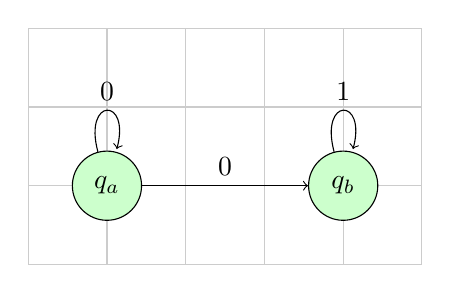
\begin{tikzpicture}[node distance=3cm,every state/.style={fill=green!20},auto]
  \draw[black!20] (-1,-1) grid (4,2);
  \node[state] (q_a) {$q_a$};
  \node[state] (q_b) [right of=q_a] {$q_b$};
  \path[->] 
  (q_a) edge node {0} (q_b)
        edge [loop above] node {0} ()
  (q_b) edge [loop above] node {1} ();
\end{tikzpicture}
\end{framed}

But, for example, the edges could be made invisible with the layer toolbar:
\begin{framed}
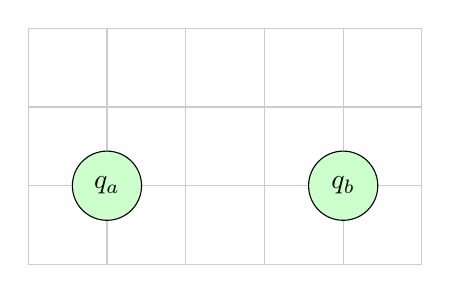
\begin{tikzpicture}[node distance=3cm,every state/.style={fill=green!20},auto]
  \draw[black!20] (-1,-1) grid (4,2);
  \node[state] (q_a) {$q_a$};
  \node[state] (q_b) [right of=q_a] {$q_b$};
\end{tikzpicture}
\end{framed}

Or the grid could be made invisible:
\begin{framed}
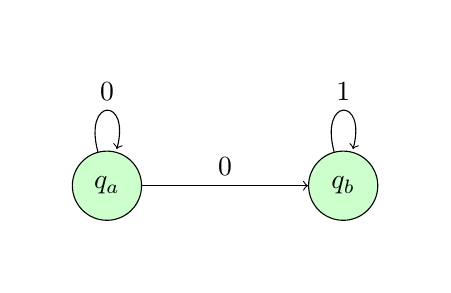
\begin{tikzpicture}[node distance=3cm,every state/.style={fill=green!20},auto]
  \draw[white!0] (-1,-1) grid (4,2);
  \node[state] (q_a) {$q_a$};
  \node[state] (q_b) [right of=q_a] {$q_b$};
  \path[->] 
  (q_a) edge node {0} (q_b)
        edge [loop above] node {0} ()
  (q_b) edge [loop above] node {1} ();
\end{tikzpicture}
\end{framed}


\subsection{Example 3: OGC and the \TikZ{} package again}
These example should show how the layers can be used within text.
\begin{lstlisting}
The following text can be toggled: 
\begin{tikzpicture}[baseline=0]
\tikzstyle{nome}=[anchor=base,outer sep=0,inner sep=0,minimum height=.45cm,minimum width=4.4cm]
\begin{ocg}{blue text}{ocblueid}{1}
  \node[nome,blue]        (p1)  {\parbox[b][][t]{4.4cm}{This text is written in blue.}};
\end{ocg}
\begin{ocg}{red text}{ocredid}{0}
  \node[overlay,nome,red] (p2)  {\parbox[b][][t]{4.4cm}{This text is written in red.}};
\end{ocg}
\end{tikzpicture}
And now the text is black again.
\end{lstlisting}

With the layer toolbar of the viewer it is possible to activate or deactivate the two layers, so there are three possibilities how it can be seen:
\begin{framed}
\noindent The following text can be toggled: \parbox[b][][t]{4.4cm}{\textcolor{blue}{This text is written in blue.}} And now the text is black again.
\end{framed}

\begin{framed}
\noindent The following text can be toggled: \parbox[b][][t]{4.4cm}{\textcolor{red}{This text is written in red.}} And now the text is black again.
\end{framed}




\begin{framed}
\noindent The following text can be toggled: 
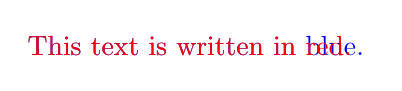
\begin{tikzpicture}[baseline=0]
\tikzstyle{nome}=[anchor=base,outer sep=0,inner sep=0,minimum height=.45cm,minimum width=4.4cm]
  \node[nome,blue]        (p1)  {\parbox[b][][t]{4.4cm}{This text is written in blue.}};
  \node[overlay,nome,red] (p2)  {\parbox[b][][t]{4.4cm}{This text is written in red.}};
\end{tikzpicture}
And now the text is black again.
\end{framed}

\newpage
\subsection{Example 4: OGC and link actions (buttons)}
Combining the  \pkg{Ti\emph{k}Z} package with buttons to show, hide, toggle or set the layers adds much possibilities how this package can be used. Here is a way to show, how a table can be made, which can be sorted by clicking on the headers.

\begin{lstlisting}
\usepackage{ocg-p}
\usepackage{tikz}           % will be needed for this example
\usepackage{datatool}   % will be needed for this example
\usepackage{booktabs}  % will be needed for this example

.
.
.

% generate database with data for the table 
\DTLnewdb{sdata}
\DTLnewrow{sdata}
\DTLnewdbentry{sdata}{Firstname}{John}
\DTLnewdbentry{sdata}{Lastname}{Doe}
\DTLnewdbentry{sdata}{Grade}{5}
\DTLnewrow{sdata}
\DTLnewdbentry{sdata}{Firstname}{Paul}
\DTLnewdbentry{sdata}{Lastname}{Bauer}
\DTLnewdbentry{sdata}{Grade}{1}
\DTLnewrow{sdata}
\DTLnewdbentry{sdata}{Firstname}{Peggy}
\DTLnewdbentry{sdata}{Lastname}{Sue}
\DTLnewdbentry{sdata}{Grade}{3}
\DTLnewrow{sdata}
\DTLnewdbentry{sdata}{Firstname}{Ever}
\DTLnewdbentry{sdata}{Lastname}{Last}
\DTLnewdbentry{sdata}{Grade}{4}
\DTLnewrow{sdata}
\DTLnewdbentry{sdata}{Firstname}{Werner}
\DTLnewdbentry{sdata}{Lastname}{Moshammer}
\DTLnewdbentry{sdata}{Grade}{1}

This table can be sorted by clicking on the headers: 

\begin{tikzpicture}
\begin{ocg}{First Name}{ocfirstid}{0}
  \node[] (p1)  {
\begin{tabular}{llc}
\toprule
\bfseries \setocgs{}{ocfirstid}{oclastid ocgradeid}{First name} 
& \bfseries \setocgs{}{oclastid}{ocfirstid ocgradeid}{Last name} 
& \bfseries \setocgs{}{ocgradeid}{ocfirstid oclastid}{Grade}
\DTLsort*{Firstname}{sdata}% sorted on the first name
\DTLforeach{sdata}{\first=Firstname, \last=Lastname,\grade=Grade}{%
\DTLiffirstrow{\\ \midrule}{\\}
\first & \last & \grade
}
\\ \bottomrule
\end{tabular}
};
\end{ocg}

\begin{ocg}{First Name}{oclastid}{1}
  \node[overlay]  (p2)  {
\begin{tabular}{llc}
\toprule
\bfseries \setocgs{}{ocfirstid}{oclastid ocgradeid}{First name} 
& \bfseries \setocgs{}{oclastid}{ocfirstid ocgradeid}{Last name} 
& \bfseries \setocgs{}{ocgradeid}{ocfirstid oclastid}{Grade}
\DTLsort*{Lastname}{sdata}% sorted on the last name
\DTLforeach{sdata}{\first=Firstname, \last=Lastname,\grade=Grade}{%
\DTLiffirstrow{\\ \midrule}{\\}
\first & \last & \grade 
}
\\ \bottomrule
\end{tabular}
};
\end{ocg}

\begin{ocg}{First Name}{ocgradeid}{0}
  \node[overlay] (p3)  {
\begin{tabular}{llc}
\toprule
\bfseries \setocgs{}{ocfirstid}{oclastid ocgradeid}{First name} 
& \bfseries \setocgs{}{oclastid}{ocfirstid ocgradeid}{Last name} 
& \bfseries \setocgs{}{ocgradeid}{ocfirstid oclastid}{Grade}
\DTLsort*{Grade}{sdata}% sorted on the grade
\DTLforeach{sdata}{\first=Firstname, \last=Lastname,\grade=Grade}{%
\DTLiffirstrow{\\ \midrule}{\\}
\first & \last & \grade
}
\\ \bottomrule
\end{tabular}
};
\end{ocg}

\end{tikzpicture}
\end{lstlisting}

\DTLnewdb{sdata}
\DTLnewrow{sdata}
\DTLnewdbentry{sdata}{Firstname}{John}
\DTLnewdbentry{sdata}{Lastname}{Doe}
\DTLnewdbentry{sdata}{Grade}{5}
\DTLnewrow{sdata}
\DTLnewdbentry{sdata}{Firstname}{Paul}
\DTLnewdbentry{sdata}{Lastname}{Bauer}
\DTLnewdbentry{sdata}{Grade}{1}
\DTLnewrow{sdata}
\DTLnewdbentry{sdata}{Firstname}{Peggy}
\DTLnewdbentry{sdata}{Lastname}{Sue}
\DTLnewdbentry{sdata}{Grade}{3}
\DTLnewrow{sdata}
\DTLnewdbentry{sdata}{Firstname}{Ever}
\DTLnewdbentry{sdata}{Lastname}{Last}
\DTLnewdbentry{sdata}{Grade}{4}
\DTLnewrow{sdata}
\DTLnewdbentry{sdata}{Firstname}{Werner}
\DTLnewdbentry{sdata}{Lastname}{Moshammer}
\DTLnewdbentry{sdata}{Grade}{1}

The output is the following table:

\begin{framed}
This table can be sorted by clicking on the headers: 

\begin{tabular}{llc}
\toprule
\bfseries First name & \bfseries Last name& \bfseries Grade
\DTLsort*{Lastname}{sdata}% sorted on the Last name
\DTLforeach{sdata}{\first=Firstname, \last=Lastname,\grade=Grade}{%
\DTLiffirstrow{\\ \midrule}{\\}
\first & \last & \grade
}
\\ \bottomrule
\end{tabular}
\end{framed}

By clicking on |Grade| in the header the table changes the sorting and looks then as follows:

\begin{framed}
This table can be sorted by clicking on the headers: 

\begin{tabular}{llc}
\toprule
\bfseries First name & \bfseries Last name& \bfseries Grade
\DTLsort*{Grade}{sdata}% sorted on the grade
\DTLforeach{sdata}{\first=Firstname, \last=Lastname,\grade=Grade}{%
\DTLiffirstrow{\\ \midrule}{\\}
\first & \last & \grade
}
\\ \bottomrule
\end{tabular}
\end{framed}

\subsection{Example 5: The ocgtabular environment}
This example does the same as the last but now by using the ocgtabular environment.

\begin{lstlisting}
\usepackage[ocgtabular]{ocg-p}
\usepackage{datatool}   % will be needed for this example
\usepackage{booktabs}  % will be needed for this example

.
.
.

% generate database with data for the table 
\DTLnewdb{sdata}
\DTLnewrow{sdata}
\DTLnewdbentry{sdata}{Firstname}{John}
\DTLnewdbentry{sdata}{Lastname}{Doe}
\DTLnewdbentry{sdata}{Grade}{5}
\DTLnewrow{sdata}
\DTLnewdbentry{sdata}{Firstname}{Paul}
\DTLnewdbentry{sdata}{Lastname}{Bauer}
\DTLnewdbentry{sdata}{Grade}{1}
\DTLnewrow{sdata}
\DTLnewdbentry{sdata}{Firstname}{Peggy}
\DTLnewdbentry{sdata}{Lastname}{Sue}
\DTLnewdbentry{sdata}{Grade}{3}
\DTLnewrow{sdata}
\DTLnewdbentry{sdata}{Firstname}{Ever}
\DTLnewdbentry{sdata}{Lastname}{Last}
\DTLnewdbentry{sdata}{Grade}{4}
\DTLnewrow{sdata}
\DTLnewdbentry{sdata}{Firstname}{Werner}
\DTLnewdbentry{sdata}{Lastname}{Moshammer}
\DTLnewdbentry{sdata}{Grade}{1}

This table can be sorted by clicking on the headers: 

\begin{ocgtabular}{llc}{sdata}{}
\toprule%
\bfseries \setocgtabularheader{Firstname}{First name}
& \bfseries   \setocgtabularheader{Lastname}{Last name} 
& \bfseries  \setocgtabularheader{Grade}{Grade}
\DTLforeach{sdata}{\first=Firstname, \last=Lastname,\grade=Grade}{%
\DTLiffirstrow{\\ \midrule}{\\}
\first & \last & \grade
}
\\ \bottomrule%
\end{ocgtabular}

\end{lstlisting}

\section{Possible future developement}

These ideas may appear in new versions of the \pkg{ocg-p} package:

\begin{itemize}
\item The package should work with dvips. There is still something wrong at the moment.
%\item The |ocg| environment should accept options like |notprintable|, |alwaysprinted|, |notinlayertoolbar| (means that the visiblity is not changeable), |%notexportable|, |alwaysexported|.
%So it is for example possible that a layer is not visible but is printed.
%\item Commands for buttons which make all layers visible or invisible.
\item The package should use |.dtx| instead of |.sty|.
\item Radio Button Groups (/RBGroups) %/RBGroups [[ 11 0 R 13 0 R]]  /ON[ 11 0 R] /OFF [13 0 R]
\end{itemize}


\section{Implementation}
The implementation is rather standard. At first main switches are defined to distinguish between the possible drivers |pdfLaTeX|, |XeLaTeX| and |dvips| (not fully implemented yet). Then the environment is defined.


\lstinputlisting[firstline=1, lastline=500]{ocg-p.sty}

%\VerbatimInput[fontsize=\footnotesize,firstline=1,lastline=320]{ocg-p.sty}


\section{Change history}

 \begin{description}
\item[0.1] Initial version, only usable with |XeLaTeX|, not based on the \pkg{ocg} package and therefore the arguments were a little bit different.

\item[0.2] The \pkg{ocg-p} package was made compatible with the \pkg{ocg} package using the same environment name and arguments and using the |aux| file in the same way. Support for |pdfLaTeX| was added. First public version.

\item[0.3] Fixed bug in |ocg| environment (missing \verb+\fi+). Fixed a bug if |XeLaTeX| is used. Nestes OCGs (layers inside another layer) are now handled as such.

\item[0.4] Removed  unnecessary \verb+\makeatletter+ and \verb+\makeatother+ commands, fixed an issue with the |beamer| class under |XeLaTeX| and other minor bugfixes. New options in the |ocg| environment. New commands for actions. New |ocgtabular| environment. 

\item[0.5] Planned: Not in a |.sty| file anymore, now using |.dtx|.

\end{description}


\end{document}